\subsection{ANALYSE AND DESCRIBE DATA REQUIREMENT}
\subsubsection{Research related systems}
Reference applications: StackOverflow and Reddit platform
\newline 
\indent Links: \href{https://stackoverflow.com/}{Stack Overflow},
\href{https://www.reddit.com/}{Reddit}

\textbf{General description about 2 applications:} Despite their different cultural orientations, Stack Overflow and Reddit share a common foundational principle: both are community-driven question-and-answer platforms that rely entirely on the power of crowdsourcing. The structure of these systems revolves around a self-moderating content selection mechanism based on voting (upvotes and downvotes), allowing the most useful and high-quality answers to rise to the top while gradually filtering out less valuable contributions. Furthermore, to manage the enormous volume of information generated by their users, both platforms employ effective domain-segmentation mechanisms through tags on Stack Overflow and subreddits on Reddit. These structures help connect users seeking information with communities that possess the relevant expertise. More importantly, the core value of these platforms extends beyond solving immediate problems for individual users. By storing, indexing, and publicly archiving discussions, they create vast knowledge repositories that can be accessed and reused by millions of future users through search engines.

% --- STACK OVERFLOW SECTION ---
\noindent \textbf{Primary Users of StackOverflow:}
\begin{itemize}
    \item \textbf{Question Askers:} Search for solutions, post technical questions with source code, and mark accepted answers.
    \item \textbf{Answer Contributors:} Provide answers, share debugging code snippets, and offer technical explanations.
    \item \textbf{Community Editors:} Vote on content, edit posts to improve clarity, and assign classification tags.
    \item \textbf{Administrators:} Moderate disputes, close duplicate or policy-violating questions, and maintain platform operations.
\end{itemize}

\noindent \textbf{Basic Business Analysis of StackOverflow:}
\begin{itemize}
    \item \textbf{Question Posting and Management:} Create titles, describe technical issues, insert formatted source code, and assign classification tags.
    \item \textbf{Answering and Technical Explanation:} Provide clear solutions, explain algorithms, and suggest optimized approaches.
    \item \textbf{Voting and Answer Acceptance:} The asker marks an accepted answer, while the community upvotes or downvotes content based on quality.
    \item \textbf{Reputation Accumulation:} The system recognizes contributions through Reputation points and badges, granting moderation privileges.
    \item \textbf{Content Moderation:} Review community edits, close duplicate topics, and remove spam.
\end{itemize}

% --- REDDIT SECTION ---
\noindent \textbf{Primary Users of Reddit:}
\begin{itemize}
    \item \textbf{Members (Redditors):} Explore feeds, participate in interest-based communities, create posts, and engage in discussions.
    \item \textbf{Community Moderators:} Establish subreddit rules, review posts, lock comments, and manage members.
    \item \textbf{Administrators (Admins):} Operate platform infrastructure, handle content safety, and enforce platform policies.
\end{itemize}


\noindent \textbf{Basic Business Analysis of Reddit:}
\begin{itemize}
    \item \textbf{Creating and Joining Subreddits:} Join or establish communities based on topics, interests, or areas of expertise.
    \item \textbf{Publishing Multi-format Content:} Share text posts, images, videos, links, or opinion polls.
    \item \textbf{Threaded Discussions:} Support multi-level commenting, enabling detailed interactions within specific conversation branches.
    \item \textbf{Voting and Karma System:} Users upvote or downvote content, while algorithms rank posts according to categories such as Hot, Top, and New.
    \item \textbf{Subreddit Moderation and Administration:} Configure keyword filters, remove posts that violate community rules, and process user reports.
\end{itemize}

\textbf{Some interfaces: }
\begin{figure}[H]
    \centering
    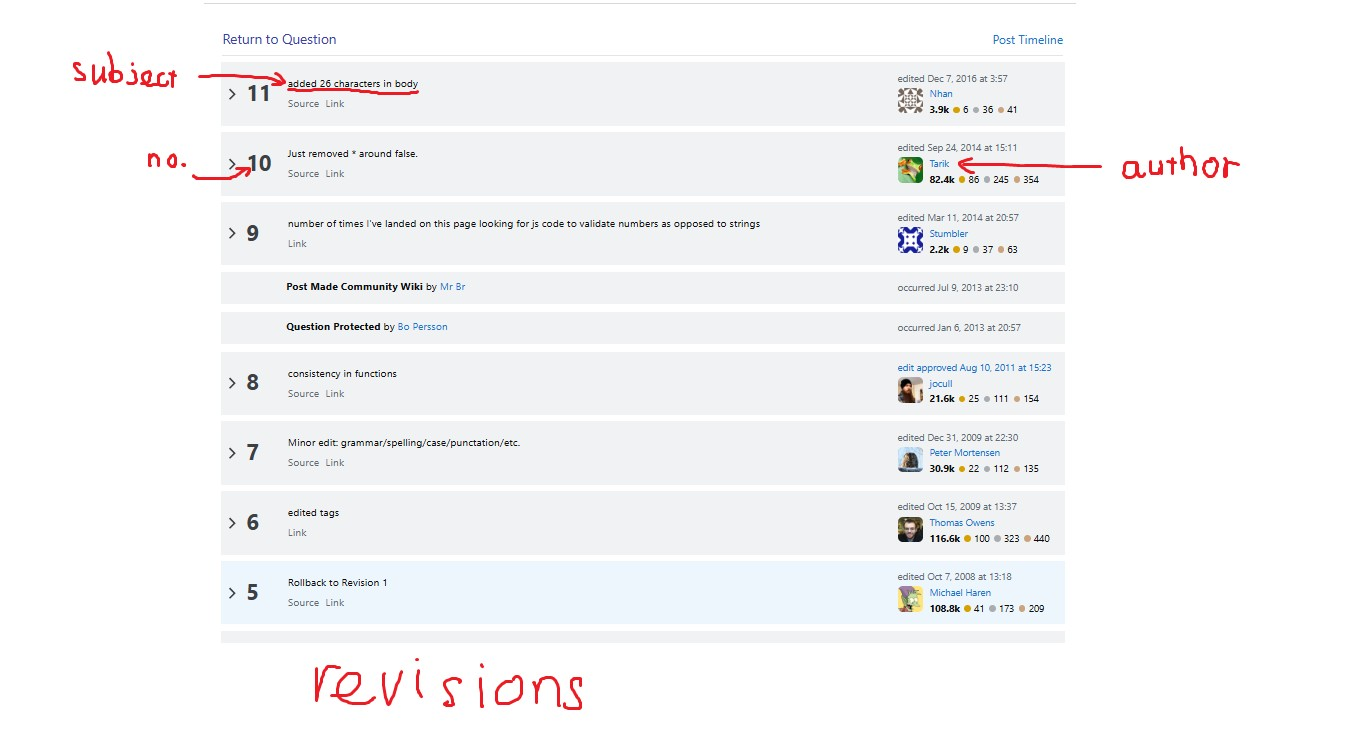
\includegraphics[width=0.9\textwidth]{lenam(1).jpg}
    \caption{Stack Overflow interface}
    \label{fig:stackoverflow_interface}
\end{figure}
\begin{figure}[H]
    \centering
    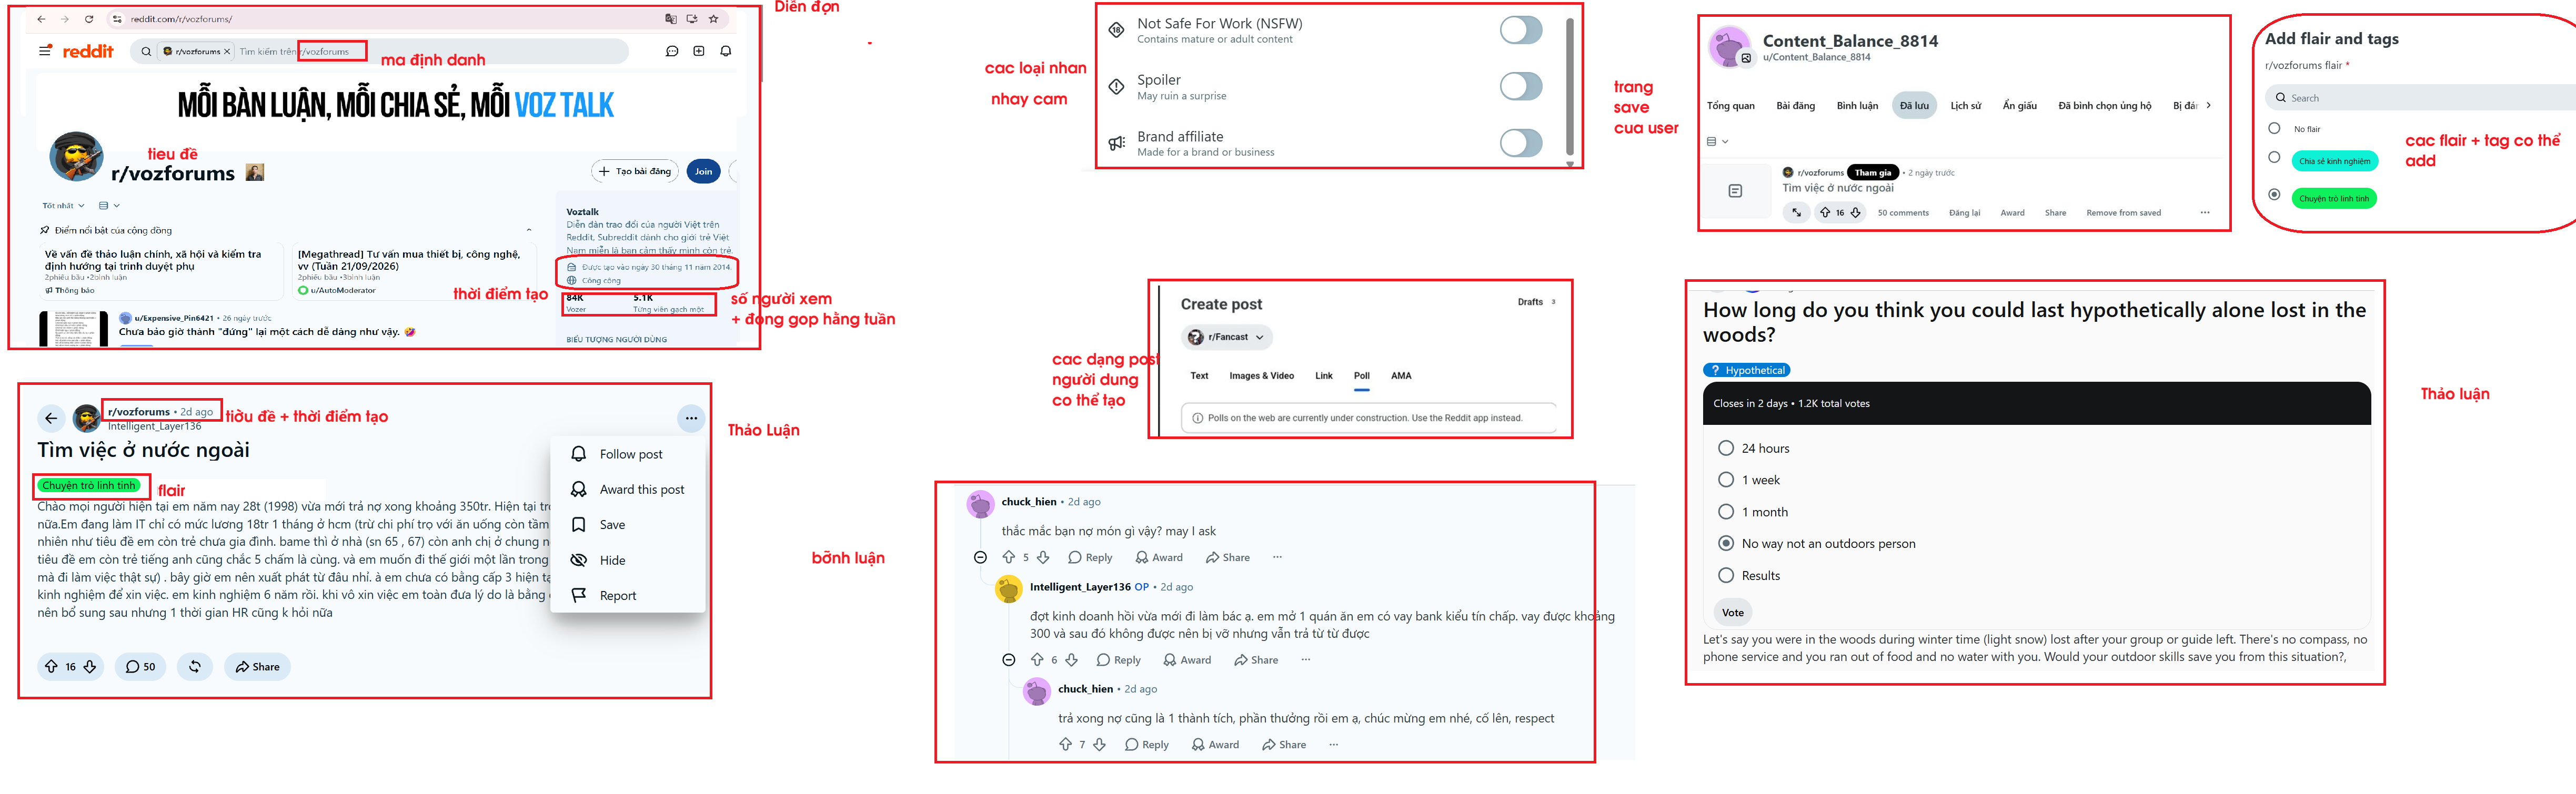
\includegraphics[width=0.9\textwidth]{../figures/hcsdl.png}
    \caption{Reddit interface}
    \label{fig:reddit_interface}
\end{figure}

\subsubsection{System description}
Team 4 proposes to develop StudentForum, an online forum system that provides a platform for students from different universities and schools to participate in communities, exchange information, ask questions, share experiences, provide feedback, and communicate with other students. The system is inspired by community-based discussion platforms such as Reddit and Stack Overflow, while being adapted to the context of student communities.

Each participating university can have its own community, where users can participate according to the requirements established by that community. The system includes students who participate in discussions, community administrators who manage individual communities, a system administrator who manages the overall platform, and students who can be assigned to manage individual forums.

A \textbf{USER} represents an account that participates in or manages activities within the StudentForum system. USER is specialized into two overlapping and total subclasses: \textbf{STUDENT} and \textbf{COMMUNITY\_ADMIN}. A STUDENT represents a student who uses the platform to participate in communities and interact with forum content, while a COMMUNITY\_ADMIN represents a user responsible for managing a particular community. The system stores common user information such as User\_ID, username, password, Email, Date\_of\_birth, Gender, and Phone. The \textbf{Phone} attribute is multivalued because a user may have multiple phone numbers. To ensure that the platform is restricted to students and authorized users, accounts representing students can only log in using a verified educational email address.

A \textbf{STUDENT} is a type of USER who participates in StudentForum and interacts with communities and discussion content. The system stores information about a student's program, representing the academic program in which the student is enrolled, such as a standard or high-quality program. Each student studies at exactly one university, while a university can have multiple students, through the STUDY\_AT relationship.

A student can become a member of multiple communities, while each community can contain multiple students through the \textbf{MEMBER OF }relationship. Through community membership, students can access forums, create posts, write comments, vote on discussion items, and interact with other participants. A student can also propose and create a forum within a community. After the forum creation request is approved by a COMMUNITY\_ADMIN, the student can be assigned as a FORUM\_ADMIN of that forum through the MANAGE relationship.

A \textbf{COMMUNITY\_ADMIN} represents a type of USER responsible for managing a particular community. Through the \textbf{CONTROL }relationship, each COMMUNITY\_ADMIN manages exactly one COMMUNITY, while a COMMUNITY can be managed by multiple COMMUNITY\_ADMINs. COMMUNITY\_ADMINs are responsible for managing community activities and reviewing requests related to the creation and management of forums within the community, they have some certain privileges. A COMMUNITY\_ADMIN does not necessarily have to be associated with the university represented by the corresponding community. For example, a COMMUNITY\_ADMIN responsible for managing the HCMUT Community may be associated with another university. Therefore, the management responsibility of a COMMUNITY\_ADMIN is determined by the community to which the administrator is assigned rather than by the university associated with the administrator's own student status.

A \textbf{SYSTEM\_ADMIN} represents an administrator responsible for managing the StudentForum platform at the system level. The system stores information about the system administrator such as SysadminID and systemAdminName. A SYSTEM\_ADMIN can \textbf{handle} administrative activities related to universities participating in StudentForum through the HANDLE relationship. The system administrator operates at the platform level and is responsible for managing system-wide activities rather than managing the content of an individual community or forum. 

A \textbf{UNIVERSITY} represents a university or educational institution participating in StudentForum. Each university is handled by exactly one SYSTEM\_ADMIN, while a SYSTEM\_ADMIN can handle multiple universities. The system stores information about each university such as Uni\_ID, Uni\_name, and uni\_description. A university can have a corresponding COMMUNITY, while each community corresponds to one university through the CORRESPOND relationship. For example, HUTECH can have a HUTECH Community and HCMUT can have an HCMUT Community. The university therefore provides the institutional context for the corresponding community in StudentForum.

A \textbf{COMMUNITY} represents the main discussion space associated with a particular university. The system stores information about a community such as Com\_name, creation\_date, and com\_description. A community can contain multiple forums through the HAS relationship, while each forum belongs to one community. A community can also have multiple participating students through the \textbf{MEMBER} OF relationship and can be managed by multiple COMMUNITY\_ADMINs through the CONTROL relationship. The system can derive the number of participants and number of community administrators from these relationships. The community provides the main environment for students to participate in discussions and access smaller forums related to different topics or interests.

A \textbf{FORUM} represents a smaller discussion space within a community and focuses on a particular topic or interest. For example, the HUTECH Community may contain forums such as “Street Food of HUTECH” or “Game Net Clubs near HUTECH”. A forum stores information such as ForumName, Description, and Creation\_date. A community can contain multiple forums, while each forum belongs to one community through the HAS relationship. A student can manage one or more forums through the \textbf{MANAGE} relationship. This relationship represents the \textbf{FORUM\_ADMIN} role. A forum can therefore have multiple FORUM\_ADMINs. A FORUM\_ADMIN does not necessarily have to be associated with the university corresponding to the forum and is responsible for managing activities and content within the corresponding forum.

Within a forum, students can create \textbf{POSTS} to ask questions, share information, discuss topics, provide feedback, or share their experiences and opinions. A post stores information such as Content, created time, and attachment information. Each post is created by one student and belongs to one forum, while a student can create multiple posts and a forum can contain multiple posts. Posts therefore serve as one of the main discussion objects through which students communicate within forums. A student can also modify a post after it has been created, and the system records the corresponding editing history through POST EDIT.

A \textbf{TAG} represents a topic or category used to classify posts. The system stores information about a tag such as TagID, Tag Name, and Description. A post must be associated with at least one tag and may have multiple tags, while a tag can be associated with multiple posts. Therefore, POST and TAG have a many-to-many relationship through the ATTACH relationship. For example, a programming-related post may be associated with tags such as “C++”, “Database”, or “Programming”, while a post about university life may have tags related to courses, campus activities, or student life. Tags allow students to classify and identify posts according to their topics.

A \textbf{COMMENT} represents a response or contribution made by a student to a discussion. A student can create multiple comments, while each comment is created by one student. A comment stores information such as Content and created date. Every comment belongs to exactly one post; a comment may additionally reply to another comment of the same post. The recursive PARENT relationship represents this reply structure, where a comment can act as a parent of multiple child comments and a child comment can have a parent comment. This allows StudentForum to support nested discussions in which students can directly respond to previous comments. Students can also modify their comments after creation, and the system records the corresponding editing history through COMMENT EDIT.

A \textbf{POST EDIT} represents a record of an editing operation performed on a post. A post can have multiple post-edit records, while each post-edit record belongs to one post through the RECORD relationship. Similarly, a COMMENT EDIT represents a record of an editing operation performed on a comment. A comment can have multiple comment-edit records, while each comment-edit record belongs to one comment through the LOG relationship. These editing records allow the system to maintain information about modifications made to posts and comments instead of only storing their latest versions.

A \textbf{DISCUSSIONITEM} represents a generalized discussion object used to associate common interactions with different types of discussion content. The DISCUSSIONITEM abstraction covers POST, COMMENT, and FORUM. This abstraction allows relationships that are applicable to different types of discussion content, such as voting and notification-related activities, to be represented without creating separate relationships for each individual content type. Each notification is ABOUT at most one discussion item

Users can also subscribe to DISCUSSIONITEMs through the \textbf{SUBSCRIBE NOTIFICATION TO} relationship to receive notifications about activities related to discussion content that they are interested in. A user can subscribe to multiple discussion items, while a discussion item can have multiple subscribers. When a user subscribes to a discussion item, the system records the corresponding subscription relationship. When relevant activities occur on a subscribed discussion item, the system can generate a NOTIFICATION for the corresponding user. A user can cancel a subscription at any time, after which the user will no longer receive notifications related to that discussion item.

The \textbf{VOTES} relationship represents the voting activity between a STUDENT and a DISCUSSION\_ITEM. A student can vote on a discussion item, while a discussion item can receive votes from multiple students. The relationship contains the upvote boolean attribute, which indicates whether the student's current vote is an upvote or a downvote, and the last\_vote\_date attribute, which records the date and time of the most recent voting action. If a student changes their vote from an upvote to a downvote or vice versa, the system updates the upvote value and last\_vote\_date of the existing voting relationship. Therefore, the system maintains the student's current voting state for each discussion item rather than treating each change as a separate voting entity.

When displaying comments within a post, the system allows users to sort comments according to creation time, number of upvotes, or number of downvotes. When sorting by upvotes or downvotes, the system calculates the corresponding number of votes associated with each comment from the voting relationship and displays comments in descending order according to the selected vote count. If multiple comments have the same vote count, the newer comment is displayed first. This allows users to identify recent or highly supported comments more easily.

The system also provides \textbf{NOTIFICATION }to inform users about activities related to their participation in StudentForum. A user can receive multiple notifications, while each notification belongs to one user through the RECEIVE relationship. A notification stores information such as id, content, noti-date, and read\_status. A notification can also be associated with a DISCUSSION\_ITEM through the ABOUT relationship. This allows the system to provide notifications concerning activities related to posts, comments, or forums. For example, a user may receive a notification when another user interacts with discussion content related to them. The read\_status attribute indicates whether the recipient has read the notification.

Overall, StudentForum integrates USER, STUDENT, COMMUNITY\_ADMIN, SYSTEM\_ADMIN, UNIVERSITY, COMMUNITY, FORUM, POST, TAG, COMMENT, POST EDIT, COMMENT EDIT, DISCUSSION\_ITEM, and NOTIFICATION, together with their corresponding relationships, to form an integrated student discussion platform. Students can participate in communities associated with different universities, access forums, create and edit posts, classify posts using tags, create and reply to comments, and express their opinions through voting. The DISCUSSION\_ITEM abstraction allows common interactions to be applied to posts, comments, and forums. COMMUNITY\_ADMIN users manage individual communities, while students assigned through the MANAGE relationship can perform the FORUM\_ADMIN role for individual forums. The SYSTEM\_ADMIN manages the platform at the system level and handles participating universities and other system-wide activities.

\subsubsection{Sematic Constraints}
\noindent\textbf{SUMMARIZE ALL THE SEMANTIC CONSTRAINTS:}

\begin{enumerate}[]
    \item \textbf{A STUDENT must log in using a verified educational email address.} The email must be valid and associated with an educational institution participating in StudentForum.
    \item A STUDENT can belong to multiple COMMUNITIes, but a student can only be considered a member of a community after satisfying that community's membership requirements.
    \item Creation\_date of a post cannot be sooner that creation\_date of that forum
    \item Only a student in the community can request to create a forum in that community
    \item No comment can reply to itself: $\text{Comment\_ID} \neq \text{Parent\_Comment\_ID}$
    \item Parent and child comments must belong to the same post
    \item A STUDENT may choose not to vote on a DISCUSSION\_ITEM. If a student votes on a discussion item, there can be at most one current voting relationship between that STUDENT and DISCUSSION\_ITEM. The student can change the vote between an upvote and a downvote, in which case the existing voting relationship is updated. If the student removes their vote, the corresponding voting relationship is deleted.
    \item \textbf{A POST or COMMENTS can be edited at most 5 times by its creator.} After the fifth edit, the system does not allow another edit.
    \item Within the same COMMUNITY, no two FORUMs may have the same ForumName. However, forums belonging to different communities may have the same ForumName.
    \item A STUDENT can edit only the POSTs or COMMENTs that they originally created.
\end{enumerate}

